\documentclass[hyperref={pdfpagelabels=false},table,10pt]{beamer}     %mathserif,
% File Name: SetUp.tex
% Function: Make main settings of the document.


%%%%%%%%%%%%%%%%%%%%%%%%%%% BEGIN-Theme-settings %%%%%%%%%%%%%%%%%%%%%%%%%%
%%%%% http://www.hartwork.org/beamer-theme-matrix/
\usetheme{default} % Set the theme of the beamer.
%\usetheme{Frankfurt}                     %% Geovani style
%\setbeamercolor{alerted text}{fg=blue}   %% Geovani style
% W/o������:default, boxes, Bergen, Madrid, Pittsburgh, Rochester
% ���������:Antibes, JuanLesPins, Montpellier��
% ��Ŀ¼(TOC)�IJ�ߵ�����: Berkeley, PaloAlto, Goettingen, Marburg, Hannover��
% ��΢��frame������:Berlin, Ilmenau, Dresden, Darmstadt, Frankfurt, Singapore, Szeged��
% ����С�ڱ���: Copenhagen, Luebeck, Malmoe, Warsaw��
%\usecolortheme{default}  % Outer color themes. Alternatives: whale, seahorse, dolphin. default, beaver
\usecolortheme{orchid}  % Inner color themes. Alternatives: lily, orchid.
\useinnertheme[shadow]{rounded}
\usefonttheme{structurebold} % Font themes. Alternatives:  default, serif, structurebold, structureitalicserif, structuresmallcapsserif
\setbeamertemplate{frametitle}
{   \begin{center}
        \insertframetitle
    \end{center}
}
\setbeamertemplate{itemize items}[default] % Alternatives: default/triangle, circle, square, ball
\setbeamertemplate{enumerate items}[default] % Alternatives: default, circle, square, ball
\setbeamertemplate{navigation symbols}{}
\setbeamertemplate{footline}[frame number]
%\setbeamertemplate{footline}{%
%  \leavevmode%
%  \hbox{%
%    \begin{beamercolorbox}[wd=.333333\paperwidth,ht=2.25ex,dp=1ex,center]{author in head/foot}%
%      \usebeamerfont{author in head/foot}\insertshortauthor~(\insertshortinstitute)
%    \end{beamercolorbox}%
%    \begin{beamercolorbox}[wd=.333333\paperwidth,ht=2.25ex,dp=1ex,center]{title in head/foot}%
%      \usebeamerfont{title in head/foot}\insertshorttitle
%    \end{beamercolorbox}%
%    \begin{beamercolorbox}[wd=.333333\paperwidth,ht=2.25ex,dp=1ex,right]{date in head/foot}%
%      \usebeamerfont{date in head/foot}\insertshortdate{}\hspace*{2em}
%      \insertframenumber{} / \inserttotalframenumber \hspace*{2ex}
%    \end{beamercolorbox}
%    }%
%  \vskip0pt%
%}
%%%%%%%%%%%%%%%%%%%%%%%%%%%% END-Theme-settings %%%%%%%%%%%%%%%%%%%%%%%%%%%


%%%%%%%%%%%%%%%%%%%%%%%%%%%%%% BEGIN-Packages %%%%%%%%%%%%%%%%%%%%%%%%%%%%%
\usepackage{amsmath,amssymb,amsfonts}
\usepackage{mathrsfs}
\usepackage{color,xcolor}
\usepackage{graphicx,subfigure}
\usepackage{clock} % Use this package to insert a clock in the beamer.
\usepackage{textcomp}
\usepackage[T1]{fontenc}
\usepackage{verbatim}
\usepackage{moreverb}
\usepackage{multirow,multicol}
%\usepackage{url}
%\usepackage[colorlinks,linkcolor=blue,citecolor=blue,urlcolor=blue]{hyperref}%[colorlinks,linkcolor=blue,citecolor=blue,urlcolor=blue]
\usepackage{CJK}
%%%%%%%%%%%%%%%%%%%%%%%%%%%%%%%% END-Packages %%%%%%%%%%%%%%%%%%%%%%%%%%%%%


% \setbeamertemplate{navigation symbols}{} % Disable the buttons at the bottom.

\graphicspath{{Figures/}} % Set the directory where figures are saved.

%\AtBeginSection{
%  \begin{frame}{Outline}
%    \tableofcontents[currentsection,hideallsubsections]
%  \end{frame}
%}
%\AtBeginSubsection{
%  \begin{frame}{Outline}
%    \tableofcontents[currentsection,currentsubsection]
%  \end{frame}
%}
\AtBeginSection{
  \begin{frame}{Outline}
  \large{
  \tableofcontents[sections={\thesection}]  }
  \end{frame}
}

%%%%%%%%%%%%%%%%%%%% BEGIN-Theorem-like Environments %%%%%%%%%%%%%%%%%%%%%
\newtheorem{mybox}{}
\newtheorem{Con}{Conjecture}[section]
\newtheorem{Thm}{Theorem}[section]
\newtheorem{Prop}{Proposition}[Thm]
% show fig and table number
\setbeamertemplate{caption}[numbered]
% show theorems and example number
\setbeamertemplate{theorems}[numbered]
%%%%%%%%%%%%%%%%%%%%% END-Theorem-like Environments %%%%%%%%%%%%%%%%%%%%%%


%%%%%%%%%%%%%%%%%%%%%%%%%% BEGIN-New Commands %%%%%%%%%%%%%%%%%%%%%%%%%%%%
\newcommand{\email}[1]{Email: \href{mailto: #1}{\tt {\color{blue}#1}}}
\newcommand{\red}{\color{red}}
\newcommand{\blue}{\color{blue}}
\newcommand{\brown}{\color{brown}}
\newcommand{\orange}{\color{orange}}
\newcommand{\yellow}{\color{yellow}}
\newcommand{\Real}{\mathbb{R}}
\newcommand{\Tran}[1]{#1^\mathrm{T}}
\newcommand{\st}{\textnormal{s.t.}}
\newcommand{\dist}{\textnormal{dist}}
\newcommand{\bc}{\begin{center}}
\newcommand{\ec}{\end{center}}
\newcommand{\tbf}{\textbf}
\newcommand{\be}{\begin{equation}}
\newcommand{\ee}{\end{equation}}
\newcommand{\ba}{\begin{array}}
\newcommand{\ea}{\end{array}}
\newcommand{\btab}{\begin{table}\begin{tabular}}
\newcommand{\etab}{\end{tabular}\end{table}}
\newcommand{\nn}{\nonumber}
\newcommand{\xn}{x_1,x_2,\ldots,x_n}
\newcommand{\framee}[2]{\frame{\frametitle{#1} #2}}
\newcommand{\reff}[1]{(\ref{#1})} % ������
\newcommand{\inner}[2]{\left\langle#1,#2\right\rangle}

%\renewcommand{\baselinestretch}{1.3}
% Ĭ��������룬������ó����˶���
\renewcommand{\raggedright}{\leftskip=0pt \rightskip=0pt plus 0cm}
\raggedright
%\large
% define Roman numbers
\makeatletter
\newcommand{\rmnum}[1]{\romannumeral #1}
\newcommand{\Rmnum}[1]{\expandafter\@slowromancap\romannumeral #1@}
\makeatother
%%%%%%%%%%%%%%%%%%%%%%%%%%%% END-New Commands %%%%%%%%%%%%%%%%%%%%%%%%%%%%


\begin{document}
\begin{CJK*}{GBK}{kai}

\title[distance geometry]{\textsc{A New Error Function and Its Application in Distance Geometry Problem}}
\author[Zhenli SHENG]{Zhenli Sheng (ʢ����)\\email: {\blue szl@lsec.cc.ac.cn}}
% \institute{Institute of Computational Mathematics and Scientific/Engineering Computing}
\institute[ICMSEC, CAS]{Institute of Computational Mathematics and Scientific/Engineering Computing,\\Chinese Academy of Sciences}
\date[]{joint work with {\blue Prof. Ya-xiang Yuan} \\\textrm{} \\January 8, 2013\\ seminar talk}
\frame{
\titlepage
}

% File Name: ThankYou.tex
% Function: Insert an Outline page.


%\section*{\textsc{Outline}}
%\begin{frame}
%\frametitle{\textsc{Outline}}
%\end{frame}

\begin{frame}
\frametitle{\textsc{Outline}}
\tableofcontents%[pausesections]
\end{frame}


\section{Problem Introduction}
\frame{
\frametitle{Distance Geometry(DG) Problem}
Find the coordinate vectors $x_{1},x_{2},\ldots,x_{n}$ that satisfy several given distances between them. \\
\textrm{}\\
\begin{itemize}%[$\blacktriangleright$]
  \item data given:
        \begin{enumerate}[--]
          \item exact distances (error-free)
          \item inexact distances (with noises)
          \item distance bounds
        \end{enumerate}
        \textrm{}\\
        \textrm{}\\
  \item applications:
        \begin{enumerate}[--]
          \item graph realization
          \item {\red protein structure determination} (3D)
          \item sensor network localization (2D)
          \item ...
        \end{enumerate}
\end{itemize}
}

\section{Related Works}
\frame{
\frametitle{Related works}
\begin{itemize}%[$\blacktriangleright$]
  \item Matrix Decomposition Method (Blumenthal 1953, Torgerson 1958)
  \item The Embedding Algorithm (Crippen, Havel 1988)
  \item Global Smoothing Algorithm (Mor\'{e}, Wu 1997)
  \item {\red Geometric Buildup Method} (Dong, Wu 2002)
  \item SDP Relaxation Method (Ye, et al., 2006)
  \item ...
\end{itemize}
}

\frame{
\frametitle{Matrix Decomposition Method}
{\red DG problem with full set of exact distances} \\
%\textrm{}\\
\small{
Given a full set of distances, $d_{i,j} = \| x_{i}-x_{j} \|, \quad i,j=1,2,\ldots,n.$ \\
\begin{itemize}%[$\blacktriangleright$]
  \item Set $x_{n} = (0,0,0\Tran)$, we have
      \begin{eqnarray}
      % \nonumber to remove numbering (before each equation)
        \nonumber d_{i,j}^{2} &=& \|x_{i}-x_{j}\|^{2} \\
        \nonumber             &=& \|x_{i}\|^{2}-2\Tran x_{i} x_{j}+\|x_{j}\|^{2} \\
                              &=& d_{i,n}^{2}-2\Tran x_{i} x_{j}+d_{j,n}^{2}, \qquad  i,j=1,2,\ldots,n-1 \label{eq1}
      \end{eqnarray} \\
      \textrm{}\\
  \item Define $ X=(x_{1},x_{2},\ldots,x_{n}\Tran)$ and $D=\{(d_{i,n}^{2}-d_{i,j}^{2}+d_{j,n}^{2})/2: i,j=1,2,\ldots,n-1\}$,  (\ref{eq1}) $\Rightarrow {\red X\Tran X=D}$.\\
      \textrm{}\\
  \item Let $D=U\Sigma\Tran U$, $V=U(:,1:3)$ and $\Lambda=\Sigma(1:3,1:3)$. Then $X = V\Lambda^{1/2}$ solves the problem. [{\blue Eckart and Young 1936}]
\end{itemize} }
}

\frame{
\frametitle{Geometric Buildup Method}
\begin{enumerate}%[$\blacktriangleright$]
  \item Find four atoms to form a base \\
        \begin{enumerate}[--]
          \item determine their coordinates to remove the possible translation and rotation/reflection
        \end{enumerate}
        \textrm{}\\
        \textrm{}\\
  \item Determine atoms one by one
        \begin{enumerate}[--]
          \item at least four distances from the undetermined atom to determined atoms are known
        \end{enumerate}
        \textrm{}\\
        \textrm{}\\
\end{enumerate}

\footnotesize{ Zachary Voller, Zhijun Wu(2012), {\blue Distance Geometry Methods for Protein Structure Determination.}}
}

\frame{
\frametitle{Determine one unknown atom}
Given four determined atoms $x_{1},x_{2},x_{3}$ and $x_{4}$, which $x_{i}=( x_{i1},x_{i2},x_{i3} \Tran)$ are known, and four {\orange exact} distances. \\
\begin{itemize}%[$\blacktriangleright$]
  \item $d_{i,j}^{2}=\|x_{i}\|^{2}-2\Tran x_{i} x_{j}+\|x_{j}\|^{2},  \qquad i=1,2,3,4.$
  \item $\Rightarrow {\red Ax_{j}=b},$ \\
        where
         $ A=2 \left(\begin{array}{ccc}
                    x_{11}-x_{21} & x_{12}-x_{22} & x_{13}-x_{23} \\
                    x_{21}-x_{31} & x_{22}-x_{32} & x_{23}-x_{33} \\
                    x_{31}-x_{41} & x_{32}-x_{42} & x_{33}-x_{43} \\
                    \end{array} \right)$ \\
         and
         $ b= \left( \begin{array}{c}
                       (\|x_{1}\|^{2}- \|x_{2}\|^{2}) -( d_{1,j}^{2}-d_{2,j}^{2} )\\
                       (\|x_{2}\|^{2}- \|x_{3}\|^{2}) -( d_{2,j}^{2}-d_{3,j}^{2} )\\
                       (\|x_{3}\|^{2}- \|x_{4}\|^{2}) -( d_{3,j}^{2}-d_{4,j}^{2} )
                     \end{array}
         \right). $ \\
  \item {\orange Inexact} distances?
\end{itemize}
}

\frame{
\frametitle{Linear and Nonlinear Least-squares Approximation}
\small{
{\red DG problem with inexact distances}\\
%\textrm{} \\
Suppose $l$ distances between the unknown atom to the determined atoms are known.
\begin{itemize}%[$\blacktriangleright$]
  \item linear least-squares
            \begin{enumerate}[--]
              \item use only the $l$ distances
              \item $ \min \|b-Ax_{j}\|     $
            \end{enumerate}
%            \textrm{}\\
%            \textrm{}\\
  \item nonlinear least-squares
            \begin{enumerate}[--]
              \item use all the distances among the $l+1$ atoms
              \item solve a matrix decomposition problem
              \item move the same points in two different reference system coincide
            \end{enumerate}
            \footnotesize{  Atilla Sit, Zhijun Wu and Ya-xiang Yuan(2009), {\blue A geometric buildup algorithm for the solution of the distance geometry problem using least-squares approximation.}}
\end{itemize} }
}


%\frame{
%\begin{figure}[htp]
%  \centering
%  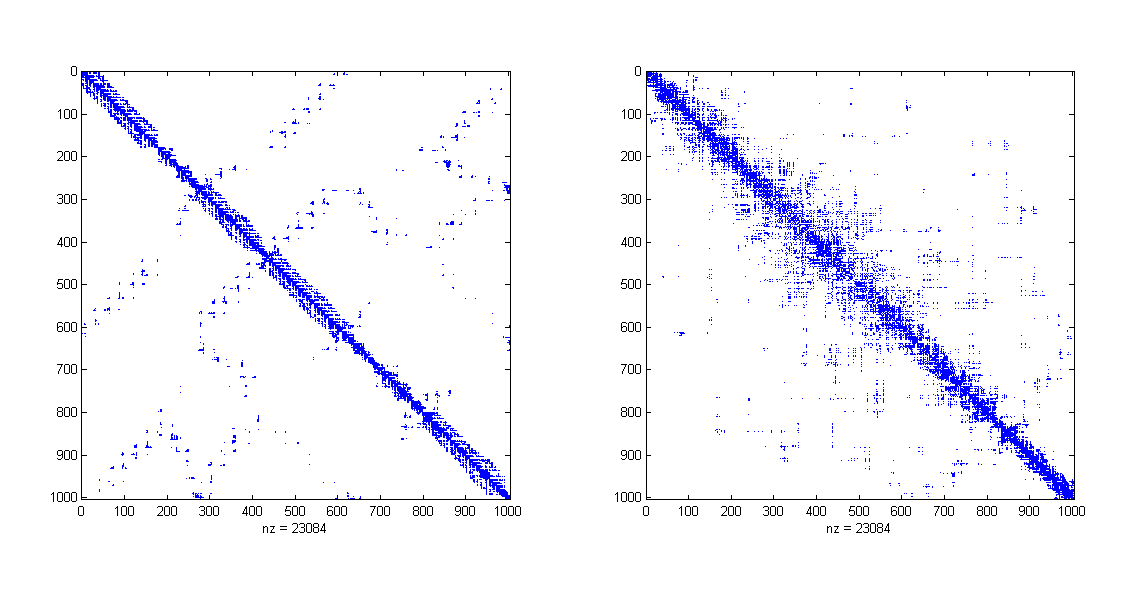
\includegraphics[width=10cm]{1AX8laplacian.png}
%  \caption{1AX8}
%\end{figure}
%}
%
%\frame{
%\frametitle{Implement Details }
%\begin{itemize}%[$\blacktriangleright$]
%  \item<2-> computational order: \\
%            \textrm{}\\
%            \begin{center}
%            \footnotesize{
%            \begin{tabular}{|c|c|c|}
%            % after \\: \hline or \cline{col1-col2} \cline{col3-col4} ...
%              \hline
%              \multicolumn{3}{|c|}{IAX8, 1003 atoms, cutoff=5{\AA}, 2.3\% exact} \\
%              \hline
%              order & RmsdError({\AA}) & CPU time (s) \\
%              \hline
%              original & 7.395926e+00 & 1.258295 \\
%              \hline
%              greedy & 9.281000e-05 & 2.346640 \\
%              \hline
%              Laplacian & 9.281000e-05 & 1.999627\\
%              \hline
%              random & 7.372537e-07 & 4.980335 \\
%                     & 1.726266e-07 & 2.946320 \\
%                     & 3.858138e-03 & 2.988656 \\
%                     & 2.437341e-08 & 3.517570 \\
%                     & 1.223379e-05 & 4.757714 \\
%                     & 1.169260e-03 & 5.339559 \\
%                     & 1.399711e-06 & 2.478225 \\
%                     & 1.771925e-05 & 4.957635 \\
%                     & 9.559394e-09 & 2.750663 \\
%                     & 8.637780e-07 & 5.196890 \\
%              \hline
%            \end{tabular} }
%            \end{center}
%  \end{itemize}
%}
%
%\frame{
%\begin{itemize}%[$\blacktriangleright$]
%  \item computational order:\\
%            \textrm{}\\
%            \begin{center}
%            \footnotesize{
%            \begin{tabular}{|c|c|c|}
%                \hline
%                \multicolumn{3}{|c|}{1MQQ, 5681 atoms, cutoff=6{\AA}, 0.75\%, exact} \\
%                \hline
%                order & RmsdError({\AA}) & CPU time (s) \\
%                \hline
%                original & 1.130061e+01 & 11.262673 \\
%                \hline
%                greedy & 4.310119e-03 & 53.904010 \\
%                \hline
%                Laplacian & 5.039401e-05 & 135.032459 \\
%                \hline
%                random & 5.315594e-03 & 23.218307 \\
%                       & 1.612265e-02 & 67.657580 \\
%                       & 2.928411e-04 & 142.834237 \\
%                       & 2.262457e-07 & 29.632780 \\
%                       & 3.823293e-06 & 70.646800 \\
%                       & 3.165929e-03 & 140.470924 \\
%                       & 8.535506e-01 & 254.812797 \\
%                       & 6.665072e-05 & 214.758550 \\
%                       & 4.334586e-01 & 141.894475 \\
%                       & 2.888975e-01 & 23.932108 \\
%                \hline
%              \end{tabular} }
%              \end{center}
%\end{itemize}
%}

%\frame{
%\begin{itemize}%[$\blacktriangleright$]
%  \item computational order:\\
%  \footnotesize{
%    \begin{tabular}{|c|c|cc|cc|}
%      \hline
%      % after \\: \hline or \cline{col1-col2} \cline{col3-col4} ...
%      PDB ID & No. of atoms & RmsdError({\AA}) & CPU time & RmsdError({\AA}) & CPU time\\
%     \hline
%      1PTQ & 402 & 6.166615e+00 & 0.527040 & 4.801191e-11 & 3.236164 \\
%      1HOE & 558 & 3.469324e-04 & 0.468773 & 3.265660e-07 & 0.915511 \\
%      1LFB & 641 & 2.143626e-02 & 0.536184 & 2.517902e-06 & 0.910246 \\
%      1PHT & 811 &  &                       & 8.865440e-07 & 1.163034 \\
%      1POA & 914 & 1.009639e+01 & 1.071874 & 3.524817e-04 & 1.875779 \\
%      1AX8 & 1003 & 7.395926e+00 & 1.014269 & 9.281000e-05 & 2.039256 \\
%      1F39 & 1534 & 2.039362e+01 & 1.541356 & 6.742977e-05 & 3.904877\\
%      1RGS & 2015 & (5)4.570301e+03 & 1.874291 &(5)8.395178e+01 & 8.853443 \\
%      1KDH & 2923 & 2.096024e+01 & 2.787796 &(1)7.433055e+05 & 31.949689\\
%      1BPM & 3672 & (3)7.641587e+05 & 3.881272 &(6)3.217206e+05 & 24.251074\\
%      1RHJ & 3740 & 2.026798e+01 & 4.451570 & & \\
%      1HQQ & 3944 & (6)1.635136e+02 & 5.424702 & &\\
%      1TOA & 4292 & (12)2.647972e+01 & 5.086191 & &\\
%      1MQQ & 5681 & 2.313884e+04 & 7.136006 & &\\
%      \hline
%    \end{tabular} }
%\end{itemize}
%}
%
%\frame{
%\begin{center}
%\footnotesize{
%\begin{tabular}{|c|c|ccc|c|ccc|}
%  \hline
%  % after \\: \hline or \cline{col1-col2} \cline{col3-col4} ...
%  PDB ID & No. &  \multicolumn{3}{c|}{greedy order} &  & \multicolumn{3}{c|}{Laplacian order} \\
%  \hline
%         &     & RmsdError({\AA}) & CPU time & NumDet & & RmsdError({\AA}) & CPU time & NumDet \\
%  \hline
%    1PTQ & 402 & 1.15e-12 & 1.22e+00 & 402 & & 8.97e-13 & 4.98e-01 & 402 \\
%    1HOE & 558 & 1.50e-12 & 8.09e-01 & 558 & & 1.08e-11 & 2.17e+00 & 558 \\
%    1LFB & 641 & 7.59e-10 & 9.10e-01 & 641 & & 1.75e-10 & 1.51e+00 & 641 \\
%    1PHT & 811 & 1.61e-11 & 1.23e+00 & 811 & & 1.67e-13 & 8.41e+01 & 4   \\
%    1POA & 914 & 6.17e-10 & 1.43e+00 & 914 & & 3.31e-11 & 1.59e+00 & 914 \\
%    1AX8 & 1003 & 1.24e-11 & 1.68e+00 & 1003 & & 4.87e-07 & 3.62e+00 & 1003 \\
%    1F39 & 1534 & 2.32e-06 & 3.86e+00 & 1534 & & 4.03e-14 & 2.93e+02 & 1534 \\
%    1RGS & 461  & 2.61e-14 & 2.11e-01 & 4    & & 3.33e-14 & 2.14e+00 & 4    \\
%    1KDH & 2846 & 7.15e-04 & 8.56e+00 & 2846 & & 1.58e-01 & 5.17e+00 & 2846 \\
%    1BPM & 3671 & 4.45e-05 & 9.03e+00 & 3671 & & 9.45e-13 & 9.92e+02 & 4    \\
%    1RHJ & 3740 & 3.47e-08 & 1.07e+01 & 3740 & & 1.00e-06 & 1.19e+01 & 3740 \\
%    1HQQ & 3944 & 4.77e-06 & 1.22e+01 & 3944 & & 2.76e+00 & 7.43e+00 & 3944 \\
%    1TOA & 4292 & 2.35e+01 & 2.79e+01 & 4292 & & 1.09e-01 & 8.93e+00 & 4292 \\
%    1MQQ & 5681 & 4.31e-03 & 4.98e+01 & 5681 & & 1.55e-02 & 5.48e+01 & 5681 \\
%  \hline
%\end{tabular} }
%\end{center}
%}

%\frame{
%\begin{figure}
%  \centering
%  \subfigure{ 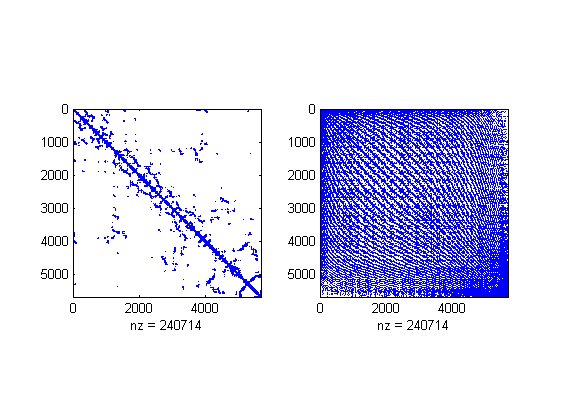
\includegraphics[width=5.5cm]{1MQQgreedyTheory.png} }
%  \subfigure{ 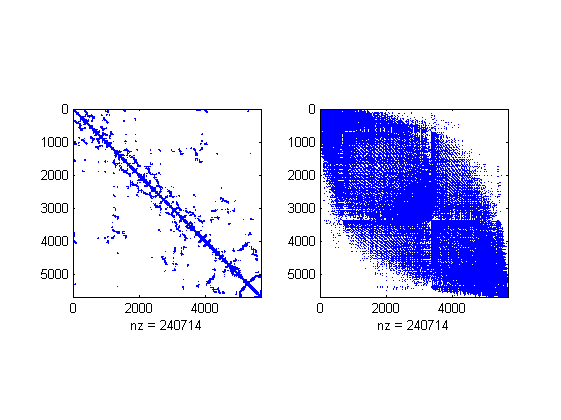
\includegraphics[width=5.5cm]{1MQQgreedyReal.png} }
%  \caption{1MQQ, greedy, theoretical VS real order}
%\end{figure}
%}

\frame{
\frametitle{Some other problems}
\begin{itemize}%[$\blacktriangleright$]
  \item Not enough bases \begin{enumerate}
              \item[--] less than four distances can be found
            \end{enumerate}
  \item Bad condition number \\% cond$(\Tran AA)>10^{6}$ \\
            \begin{enumerate}
              \item[--] which means the bases are almost in the same plane! \\
            \centering $\Uparrow$ \\
            computational issue
            \end{enumerate}

  \item $\rightsquigarrow$ Move to the last
\end{itemize}
}

\section{Distributed Geometric Buildup Method}
\frame{
\frametitle{Motivation}
\centering
\footnotesize{
\begin{tabular}{|r|r|r|r|}
    \hline
     Itr &   RmsdError({\AA}) &     Itr &   RmsdError({\AA}) \\
     \hline
     300 & 1.02e-12 & 3000 & 1.19e-04 \\
     600 & 1.81e-10 & 3300 & 3.48e-04 \\
     900 & 2.06e-07 & 3600 & 1.95e-03 \\
    1200 & 6.69e-07 & 3900 & 1.97e-03 \\
    1500 & 3.36e-06 & 4200 & 2.16e-03 \\
    1800 & 4.68e-06 & 4500 & 2.23e-03 \\
    2100 & 7.87e-06 & 4800 & 2.79e-03 \\
    2400 & 2.06e-05 & 5100 & 3.08e-03 \\
    2700 & 6.99e-05 & 5400 & 4.28e-03 \\
     \hline
\end{tabular} } \\

\begin{itemize}
  \item 1MQQ, 5681 atoms, cutoff=6{\AA}, 0.75\%, exact distances, Buildup Method
  \item {\red Rounding error accumulates!}
\end{itemize}
}

\frame{
\frametitle{Idea of distributed method}
The idea is quite simple. It is a "Divide and Conquer" method. \\
\textrm{}\\
\begin{enumerate}%[$\blacktriangleright$]
  \item Divide the whole protein into small patches with some overlaps
  \item Apply Geometric Buildup Method at each patch
  \item Make use of the overlap to stitch them together
\end{enumerate}
}

\frame{
\frametitle{How to divide}
\begin{itemize}%[$\blacktriangleright$]
  \item {\blue symrcm}: minimize the bandwidth \\
       \begin{figure}[htp]
             \centering
             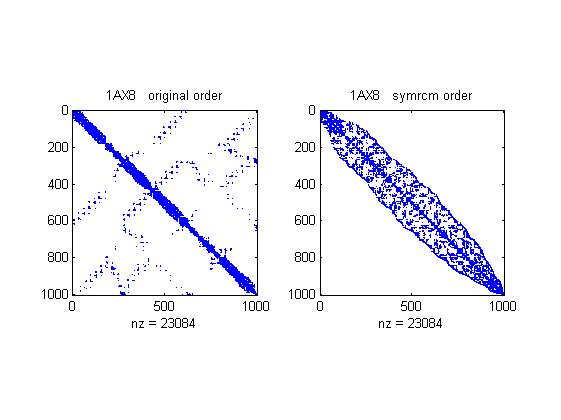
\includegraphics[totalheight=2 in]{1AX8symrcm.png}
       \end{figure}
  \scriptsize{  Pratik Biswas, Kim-Chuan Toh and Yinyu Ye(2007), {\blue A Distributed SDP Approach for Large-scale Noisy Anchor-free Graph Realization with Application to Molecular Conformation.}}
\end{itemize}
}

\frame{
\frametitle{Divide(Cont'd): Laplacian Matrix}
\small{
Given a graph $(V,E)$, define its Laplacian matrix by $L$, whose entries $l_{i,j}$ are given by
\begin{itemize}%[$\blacktriangleright$]
  \item \begin{equation*}
             l_{i,j}=\left \{ \begin{array}{cll}
                      deg(v_{i}) & \textrm{if  } i=j, & \qquad  \rightarrow -sum(L(i,:))\\
                      -1         & \textrm{if  } (i,j)\in E, & \qquad \rightarrow {\red -exp(-d_{i,j}^{2}/2 ) }\\
                      0          & \textrm{otherwise}. &  \\
                              \end{array}
                     \right.
            \end{equation*}
            \textrm{}\\
            \textrm{}\\
            $L=D-A$, where D is degree matrix, and A is its adjacency matrix.
            \textrm{}\\
            \textrm{}\\
  \item Properties:
            \begin{enumerate}[--]
              \item L is always positive-semidefinite.
              \item 0 is always its eigenvalue and its corresponding eigenvector is $(1,1,\ldots,1\Tran)$.
              \item The number of times 0 appears as an eigenvalue in the Laplacian is the number of connected components in the graph.
            \end{enumerate}
\end{itemize} }
}

\frame{
\frametitle{Eigenvector of smallest nonzero eigenvalue}
\begin{figure}[htp]
    \centering
    \subfigure{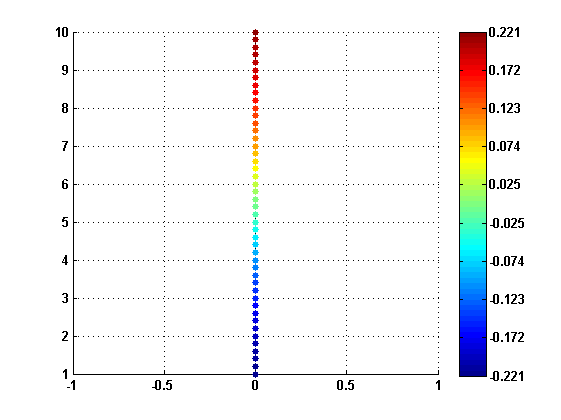
\includegraphics[width=4.5cm]{line.png} }
    \subfigure{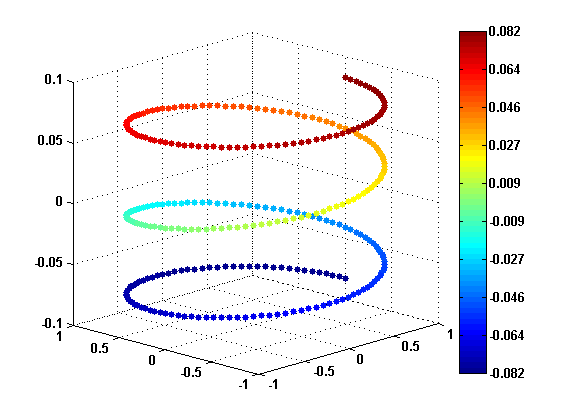
\includegraphics[width=4.5cm]{helix.png} }
    \subfigure{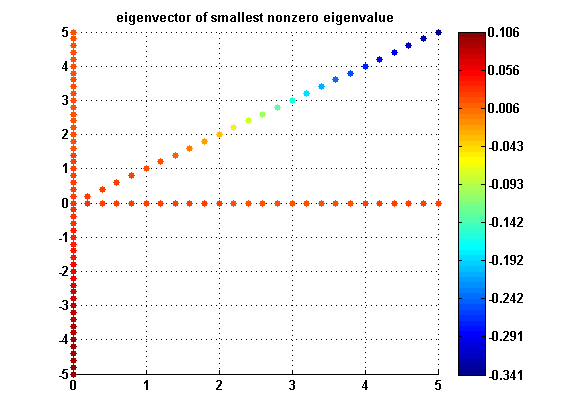
\includegraphics[width=4.5cm]{piecewise.png} }
    \subfigure{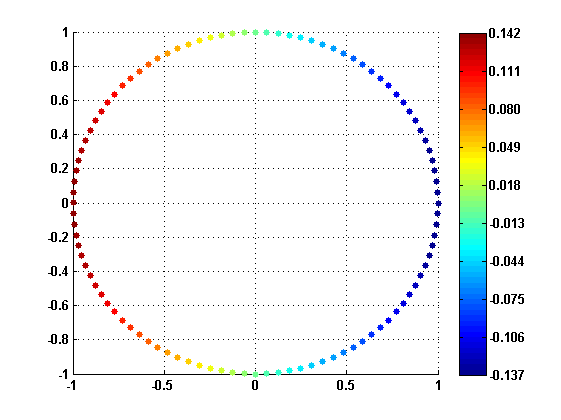
\includegraphics[width=4.5cm]{circle.png} }
\end{figure}
}

\frame{
\frametitle{a Conjecture}
%\footnotesize{
\begin{Con}
Given a graph $(V,E)$, its Laplacian matrix is defined as before, then the eigenvector of the smallest nonzero eigenvalue, which can be viewed as a function of the vertexes, monotonically decrease or increase along the main trend/direction of the graph.
\end{Con}
\begin{figure}[htp]
  \centering
  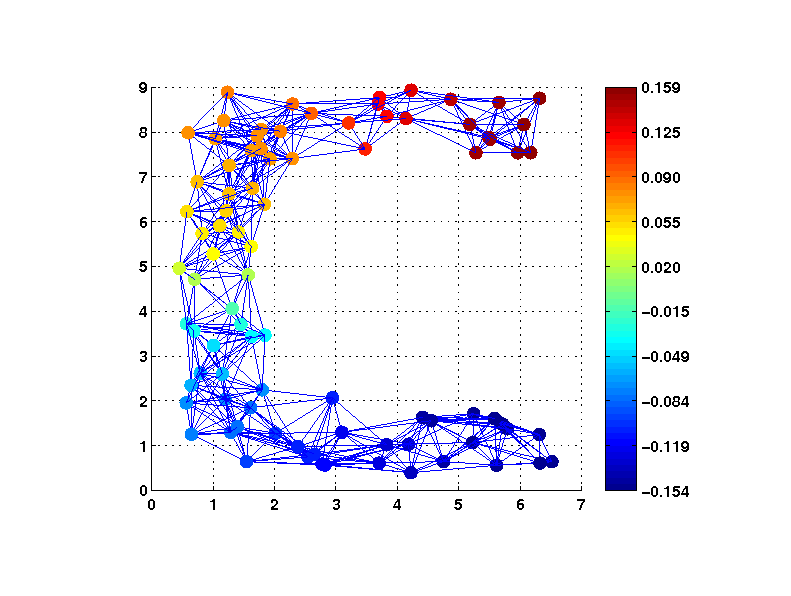
\includegraphics[width=6cm]{eigenone.png}
\end{figure}
}
%}

\frame{
\frametitle{How to stitch}
\footnotesize{
Given two 3D point sets $\{p_{i}\}$ and $\{q_{i}\}$, $i=1,2,\ldots,k$.
\begin{itemize}%[$\blacktriangleright$]
  \item  \begin{align}
               \nonumber \min_{R,T} \quad& \sum_{i=1}^{k} \| p_{i}- (Rq_{i}+T) \|_{2}^{2} \\
                         \st \quad & \Tran RR =I.
             \end{align}
  \item T: make their geometric center coincide
  \item R: \begin{align}\label{stitch}
                \nonumber \min_{R} \quad& \| P- RQ \|_{F}^{2} \\
                          \st \quad & \Tran RR =I.
               \end{align}
  Let $C=P\Tran Q$, and $C=U\Sigma\Tran V$, then $R=V\Tran U$ solves (\ref{stitch}).
  [{\blue Matrix Computation, Golub}]
  \item Remark: a fundamental problem in {\orange Machine Intelligence} and {\orange Optical Science}.
\end{itemize} }
}

\frame{
\frametitle{Algorithm framework}
\rule{\textwidth}{1pt}
\footnotesize{
\texttt{  Distributed Geometric Buildup Method for Protein Structure Determination}}
\rule{\textwidth}{0.5pt}
%\scriptsize{
\begin{enumerate}[1.]
  \item Initialize, set parameters: PatchNum, MaxItr
  \item Find four atoms that are not in the same plane, determine their coordinates with the distances among them.
  \item Construct the Laplacian matrix, sort all the atoms according to eigenvector corresponding to its minimal nonzero eigenvalue, divide the whole protein into several small patches.
  \item Solve problem on each patch with Buildup Method.
  \item Stitch all the patches together.
\end{enumerate}
\rule{\textwidth}{1pt}
}

\frame{
\frametitle{Numerical experiments}
\begin{itemize}
  \item Download structure data from Protein Data Bank(PDB), obtain the original coordinates X.
  \item Use \emph{{\blue disk graph model}} to construct distance matrix, usually set cutoff as 5{\AA} or 6{\AA}.
  \item Solve the problem with our algorithm to get Computed coordinates Y, then compare it with X, using the criteria defined as below,
        $$ RMSD(X,Y) = \min_{Q,T}\|X-YQ-T\|_{F}/\sqrt{n} $$
\end{itemize}
}

\frame{
\frametitle{PDB file}
\begin{figure}
  \centering
  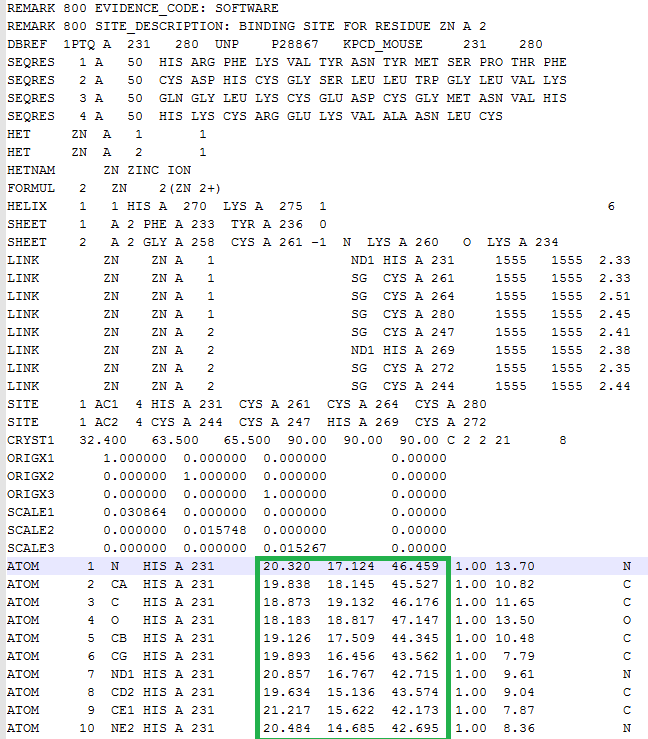
\includegraphics[totalheight=2.7 in]{PDBfile1PTQ.png}
\end{figure}
\begin{center}
  \footnotesize{1PTQ.pdb}
\end{center}
}

\frame{
\frametitle{Data information}
\centering
\scriptsize{
\begin{tabular}{|l|r||c|c||c|c|}
  \hline
  \multicolumn{6}{|c|}{exact distances} \\
  \hline
  % after \\: \hline or \cline{col1-col2} \cline{col3-col4} ...
  PdbID & Num & cutoff & degree & cutoff & degree \\
  \hline
  1PTQ &  402 & 5 & 5.46\% & 6 & 8.79\%  \\
  1HOE &  558 & 5 & 4.05\% & 6 & 6.55\%  \\
  1LFB &  641 & 5 & 3.40\% & 6 & 5.57\%  \\
  1PHT &  811 & 5 & 3.35\% & 6 & 5.37\%  \\
  1POA &  914 & 5 & 2.51\% & 6 & 4.07\%  \\
  1AX8 & 1003 & 5 & 2.30\% & 6 & 3.74\%  \\
  1F39 & 1534 & 5 & 1.47\% & 6 & 2.43\%  \\
  1RGS & 2015 & 5 & 1.12\% & 6 & 1.87\%  \\
  1KDH & 2846 & 5 & 0.83\% & 6 & 1.36\%  \\
  1BPM & 3671 & 5 & 0.66\% & 6 & 1.12\%  \\
  1RHJ & 3740 & 5 & 0.65\% & 6 & 1.10\%  \\
  1HQQ & 3944 & 5 & 0.60\% & 6 & 1.00\%  \\
  1TOA & 4292 & 5 & 0.56\% & 6 & 0.94\%  \\
  1MQQ & 5681 & 5 & 0.44\% & 6 & 0.75\%  \\
  \hline
\end{tabular}     } \\

\begin{flushleft}
    We test these 14 proteins which were used in Prof. Ye' paper as mentioned before. \\
    Notice that the atom number of these proteins varies from hundreds to more that five thousand.
\end{flushleft}
}

\frame{
\frametitle{Computational order}
  \centering
\tiny{
\begin{tabular}{|l|r||r|r||r|r||r|r||r|r|}
  \hline
  \multicolumn{10}{|c|}{cutoff=6{\AA}, exact distances, Buildup Method, {\red 'linear'}} \\
  \hline
  % after \\: \hline or \cline{col1-col2} \cline{col3-col4} ...
   PDB & Total&  Rmsd    & CPU   &   Rmsd   & CPU   &  Rmsd   & CPU  &  Rmsd   & CPU  \\
   ID  & Num  &  Error     & time  &   Error    & time  &  Error    & time &  Error    & time \\
   \hline
  \multicolumn{2}{|c||}{}& \multicolumn{2}{c||}{original} & \multicolumn{2}{c||}{{\blue greedy}} & \multicolumn{2}{c||}{randperm} & \multicolumn{2}{c|}{randperm}\\
  \hline
  1PTQ &  402 & 8.02e-12 & 0.40 & 1.15e-12 &  0.43 & 9.35e-13 &   0.56 & 6.21e-11 &   0.52  \\
  1HOE &  558 & 2.13e-12 & 0.57 & 1.50e-12 &  0.69 & 2.15e-10 &   1.24 & 1.75e-08 &   0.75  \\
  1LFB &  641 & 1.16e-10 & 0.68 & 7.59e-10 &  0.81 & 1.98e-08 &   1.46 & 5.67e-09 &   1.03  \\
  1PHT &  811 & 1.38e-09 & 0.97 & 1.61e-11 &  1.06 & 2.24e-09 &   1.23 & 4.43e-11 &   1.77  \\
  1POA &  914 & 4.53e-10 & 1.01 & 6.17e-10 &  1.26 & 1.53e-11 &   1.90 & 2.42e-11 &   2.74  \\
  1AX8 & 1003 & 3.74e-06 & 1.22 & 1.24e-11 &  1.49 & 8.74e-11 &   2.07 & 3.84e-09 &   3.11  \\
  1F39 & 1534 & 2.52e-07 & 1.90 & 2.32e-06 &  3.52 & 4.09e-03 &   6.90 & 7.17e-07 &   2.88  \\
  1RGS & 2015 & 2.24e-02 & 2.54 & 1.08e-01 &  7.65 & 3.34e-04 &   7.48 & 8.68e-04 &   8.84  \\
  1KDH & 2846 & 1.45e-03 & 3.74 & 7.15e-04 &  7.71 & 2.34e-03 &  42.33 & 2.12e-04 &  18.08  \\
  1BPM & 3671 & 6.38e-02 & 5.70 & 4.45e-05 &  9.00 & 8.90e-05 &  16.24 & 7.51e-05 &  21.17  \\
  1RHJ & 3740 & 7.07e+00 & 6.12 & 3.47e-08 &  9.83 & 6.92e-05 & 113.34 & 4.55e-07 &  67.71  \\
  1HQQ & 3944 & 2.03e-03 & 6.58 & 4.77e-06 & 11.69 & 8.07e-05 &  22.15 & 9.26e-04 &  40.18  \\
  1TOA & 4292 & 2.88e+00 & 6.58 & 2.35e+01 & 26.36 & 1.47e-05 &  67.02 & 6.64e+01 &  65.18  \\
  1MQQ & 5681 & 1.13e+01 & 9.52 & 4.31e-03 & 46.41 & 1.05e+01 &  21.84 & 1.80e+00 &  82.65  \\
  \hline
\end{tabular} }  
}

\frame{
\frametitle{Computational order (Cont'd)}
  \centering
\tiny{
\begin{tabular}{|l|r||r|r||r|r||r|r||r|r|}
  \hline
  \multicolumn{10}{|c|}{cutoff=6{\AA}, exact distances, Buildup Method, {\red 'nonlinear'}} \\
  \hline
  % after \\: \hline or \cline{col1-col2} \cline{col3-col4} ...
   PDB & Total&  Rmsd    & CPU   &   Rmsd   & CPU   &  Rmsd   & CPU  &  Rmsd   & CPU  \\
   ID  & Num  &  Error     & time  &   Error    & time  &  Error    & time &  Error    & time \\
   \hline
  \multicolumn{2}{|c||}{}& \multicolumn{2}{c||}{original} & \multicolumn{2}{c||}{{\blue greedy}} & \multicolumn{2}{c||}{randperm} & \multicolumn{2}{c|}{randperm}\\
  \hline
  1PTQ &  402 & 1.34e-13 &  0.59 & 2.26e-14 &  0.98 & 5.56e-14 &   0.88 & 6.89e-14 &    0.88  \\
  1HOE &  558 & 3.21e-13 &  0.92 & 7.80e-14 &  1.13 & 1.05e-13 &   1.10 & 7.34e-14 &    1.11  \\
  1LFB &  641 & 5.53e-14 &  0.94 & 1.42e-13 &  1.18 & 4.96e-14 &   1.40 & 1.90e-13 &    1.49  \\
  1PHT &  811 & 7.29e-13 &  1.52 & 6.04e-14 &  1.65 & 1.19e-13 &   1.71 & 2.20e-13 &    1.83  \\
  1POA &  914 & 1.56e-13 &  1.41 & 9.14e-14 &  1.69 & 2.60e-13 &   3.26 & 8.53e-14 &    2.16  \\
  1AX8 & 1003 & 8.16e-13 &  1.68 & 6.28e-14 &  2.71 & 2.07e-13 &   4.31 & 8.01e-14 &    2.56  \\
  1F39 & 1534 & 2.52e-13 &  2.53 & 7.65e-13 &  4.69 & 5.23e-13 &   6.14 & 1.35e-12 &   18.56  \\
  1RGS & 2015 & 1.93e-12 &  3.37 & 6.66e-13 &  8.61 & 3.20e-12 &   5.39 & 1.14e-11 &   17.50  \\
  1KDH & 2846 & 2.31e-11 &  5.09 & 8.43e-13 & 10.20 & 6.36e-13 &  10.63 & 1.58e-10 &   16.19  \\
  1BPM & 3671 & 1.99e-11 &  7.16 & 1.01e-12 & 14.44 & 1.11e-12 &  15.22 & 1.84e-12 &  171.51  \\
  1RHJ & 3740 & 2.27e-10 &  7.65 & 2.25e-12 & 12.71 & 2.10e-12 &  49.17 & 1.03e-12 &   39.95  \\
  1HQQ & 3944 & 4.66e-11 &  8.47 & 2.73e-12 & 14.25 & 8.22e-13 &  16.85 & 2.03e-12 &   93.09  \\
  1TOA & 4292 & 1.19e-09 &  8.74 & 7.90e-11 & 29.27 & 6.83e-11 & 115.35 & 2.61e-12 &   54.58  \\
  1MQQ & 5681 & 4.03e-08 & 12.59 & 4.21e-11 & 54.21 & 6.95e-10 & 367.92 & 3.61e-11 &   94.60  \\
  \hline
\end{tabular}  }   \\

\begin{center}
  \scriptsize{From now on, we use {\red greedy order} to implement our algorithm.}
\end{center}
}

\frame{
\frametitle{Linear VS Nonlinear}
\centering
\scriptsize{
\begin{tabular}{|l|r||r|r|r||r|r|r|}
  \hline
  \multicolumn{8}{|c|}{cutoff={\red 5}{\AA}, exact distances, Buildup Method} \\
  \hline
   PDB & Total&  RmsdError({\AA})  & CPU   &  Determined &  RmsdError({\AA})  & CPU   &  Determined  \\
   ID  & Num  &           & time  &  Num &           & time  &  Num  \\
   \hline
  \multicolumn{2}{|c||}{}& \multicolumn{3}{c||}{{\blue linear}} & \multicolumn{3}{c|}{{\blue nonlinear}} \\
  \hline
  1PTQ &  402 & 4.80e-11 &  0.49 &  402 & 2.05e-14 &  0.59 &  402  \\
  1HOE &  558 & 3.27e-07 &  0.85 &  558 & 6.52e-14 &  0.93 &  558  \\
  1LFB &  641 & 2.52e-06 &  0.85 &  641 & 3.49e-14 &  0.96 &  641  \\
  1PHT &  811 & 8.87e-07 &  1.14 &  806 & 2.52e-13 &  1.45 &  806  \\
  1POA &  914 & 3.52e-04 &  1.62 &  914 & 3.23e-13 &  1.96 &  914  \\
  1AX8 & 1003 & 9.28e-05 &  1.89 & 1003 & 7.15e-14 &  2.16 & 1003  \\
  1F39 & 1534 & 6.74e-05 &  3.74 & 1534 & 8.26e-14 &  3.86 & 1534  \\
  1RGS & 2015 & 8.40e+01 &  7.67 & 2010 & 4.46e-13 &  8.22 & 2010  \\
  1KDH & 2846 & 7.43e+05 & 29.14 & 2845 & 1.03e-11 & 28.05 & 2846  \\
  1BPM & 3671 & 3.22e+05 & 18.45 & 3665 & 2.86e-11 & 13.81 & 3668  \\
  1RHJ & 3740 & 1.83e+05 & 28.70 & 3734 & 1.56e-12 & 25.75 & 3740  \\
  1HQQ & 3944 & 2.85e+01 & 17.31 & 3938 & 2.46e-13 & 20.23 & 3938  \\
  1TOA & 4292 & 1.08e+03 & 22.30 & 4280 & 2.90e-12 & 26.82 & 4280  \\
  1MQQ & 5681 & 2.81e+00 & 35.01 & 5681 & 7.47e-13 & 35.73 & 5681  \\
  \hline
\end{tabular}  } \\

\begin{center}
  nonlinear: generally, a little more time, much more accurate!
\end{center}
}

\frame{
\frametitle{Linear VS Nonlinear (Cont'd)}
\centering
\scriptsize{
\begin{tabular}{|l|r||r|r|r||r|r|r|}
  \hline
  \multicolumn{8}{|c|}{cutoff={\red 6}{\AA}, exact distances, Buildup Method} \\
  \hline
  % after \\: \hline or \cline{col1-col2} \cline{col3-col4} ...
   PDB & Total&  RmsdError({\AA})  & CPU   &  Determined &  RmsdError({\AA})  & CPU   &  Determined  \\
   ID  & Num  &           & time  &  Num &           & time  &  Num  \\
   \hline
  \multicolumn{2}{|c||}{}& \multicolumn{3}{c||}{{\blue linear}} & \multicolumn{3}{c|}{{\blue nonlinear}} \\
  \hline
  1PTQ &  402 & 1.15e-12 &  0.43 &  402 & 2.26e-14 &  0.98 &  402  \\
  1HOE &  558 & 1.50e-12 &  0.69 &  558 & 7.80e-14 &  1.13 &  558  \\
  1LFB &  641 & 7.59e-10 &  0.81 &  641 & 1.42e-13 &  1.18 &  641  \\
  1PHT &  811 & 1.61e-11 &  1.06 &  811 & 6.04e-14 &  1.65 &  811  \\
  1POA &  914 & 6.17e-10 &  1.26 &  914 & 9.14e-14 &  1.69 &  914  \\
  1AX8 & 1003 & 1.24e-11 &  1.49 & 1003 & 6.28e-14 &  2.71 & 1003  \\
  1F39 & 1534 & 2.32e-06 &  3.52 & 1534 & 7.65e-13 &  4.69 & 1534  \\
  1RGS & 2015 & 1.08e-01 &  7.65 & 2015 & 6.66e-13 &  8.61 & 2015  \\
  1KDH & 2846 & 7.15e-04 &  7.71 & 2846 & 8.43e-13 & 10.20 & 2846  \\
  1BPM & 3671 & 4.45e-05 &  9.00 & 3671 & 1.01e-12 & 14.44 & 3671  \\
  1RHJ & 3740 & 3.47e-08 &  9.83 & 3740 & 2.25e-12 & 12.71 & 3740  \\
  1HQQ & 3944 & 4.77e-06 & 11.69 & 3944 & 2.73e-12 & 14.25 & 3944  \\
  1TOA & 4292 & 2.35e+01 & 26.36 & 4292 & 7.90e-11 & 29.27 & 4292  \\
  1MQQ & 5681 & 4.31e-03 & 46.41 & 5681 & 4.21e-11 & 54.21 & 5681  \\
  \hline
\end{tabular}  } \\

\begin{center}
  nonlinear: generally, a little more time, much more accurate!\\
  From now on, we use {\blue nonlinear} least squares to determine the new point.
\end{center}
}

\frame{
\frametitle{distributed: symrcm VS Laplacian}
\centering
\scriptsize{
\begin{tabular}{|l|r||r|r|r||r|r|r|}
  \hline
  \multicolumn{8}{|c|}{cutoff=6{\AA}, exact distances} \\
  \hline
  % after \\: \hline or \cline{col1-col2} \cline{col3-col4} ...
   PDB & Total&  RmsdError({\AA})  & CPU   &  Determined &  RmsdError({\AA})  & CPU   &  Determined  \\
   ID  & Num  &           & time  &  Num &           & time  &  Num  \\
  \hline
  \multicolumn{2}{|c||}{} & \multicolumn{3}{c||}{{\blue symrcm}} & \multicolumn{3}{c|}{{\blue Laplacian}} \\
  \hline
  1PTQ &  402 & 2.24e-14 &  0.69 &  402 & 3.54e-14 &  0.62 &  402  \\
  1HOE &  558 & 2.28e-13 &  0.95 &  558 & 8.76e-14 &  1.03 &  558  \\
  1LFB &  641 & 7.75e-14 &  1.04 &  641 & 1.43e-13 &  1.08 &  641  \\
  1PHT &  811 & 7.08e-14 &  1.61 &  811 & 1.08e-12 &  1.59 &  811  \\
  1POA &  914 & 1.39e-13 &  1.71 &  914 & 1.80e-13 &  1.73 &  914  \\
  1AX8 & 1003 & 2.62e-13 &  2.08 & 1003 & 1.04e-13 &  1.94 & 1003  \\
  1F39 & 1534 & 9.30e-14 &  3.09 & 1534 & 1.41e-13 &  3.09 & 1534  \\
  1RGS & 2015 & 1.47e-12 &  4.21 & 2015 & 1.03e-12 &  4.61 & 2015  \\
  1KDH & 2846 & 4.30e-13 &  6.51 & 2846 & 1.25e-12 &  6.09 & 2846  \\
  1BPM & 3671 & 2.35e+02 &  8.05 & 3671 & 3.58e-13 &  8.14 & 3671  \\
  1RHJ & 3740 & 1.36e-12 &  8.56 & 3740 & 6.69e-11 &  8.60 & 3740  \\
  1HQQ & 3944 & 1.02e+06 & 10.21 & 3944 & 4.29e-13 &  8.58 & 3944  \\
  1TOA & 4292 & 8.41e+06 &  9.24 & 4292 & 1.92e-12 &  9.51 & 4292  \\
  1MQQ & 5681 & 2.19e+01 & 14.89 & 5681 & 3.22e-12 & 13.33 & 5681  \\
  \hline
\end{tabular}  } \\

\begin{center}
  Laplacian: almost the same time, much more accurate!
\end{center}
}

\frame{
\frametitle{Buildup VS Distributed Buildup}
\centering
\scriptsize{
\begin{tabular}{|l|r||r|r|r||r|r|r|}
  \hline
  \multicolumn{8}{|c|}{cutoff=6{\AA}, exact distances} \\
  \hline
  % after \\: \hline or \cline{col1-col2} \cline{col3-col4} ...
   PDB & Total&  RmsdError({\AA})  & CPU   &  Determined &  RmsdError({\AA})  & CPU   &  Determined  \\
   ID  & Num  &           & time  &  Num &           & time  &  Num  \\
  \hline
  \multicolumn{2}{|c||}{} & \multicolumn{3}{c||}{{\blue Buildup}} & \multicolumn{3}{c|}{{\blue Distributed Buildup}} \\
  \hline
  1PTQ &  402 & 2.26e-14 &  0.98 &  402 & 3.54e-14 &  0.62 &  402  \\
  1HOE &  558 & 7.80e-14 &  1.13 &  558 & 8.76e-14 &  1.03 &  558  \\
  1LFB &  641 & 1.42e-13 &  1.18 &  641 & 1.43e-13 &  1.08 &  641  \\
  1PHT &  811 & 6.04e-14 &  1.65 &  811 & 1.08e-12 &  1.59 &  811  \\
  1POA &  914 & 9.14e-14 &  1.69 &  914 & 1.80e-13 &  1.73 &  914  \\
  1AX8 & 1003 & 6.28e-14 &  2.71 & 1003 & 1.04e-13 &  1.94 & 1003  \\
  1F39 & 1534 & 7.65e-13 &  4.69 & 1534 & 1.41e-13 &  3.09 & 1534  \\
  1RGS & 2015 & 6.66e-13 &  8.61 & 2015 & 1.03e-12 &  4.61 & 2015  \\
  1KDH & 2846 & 8.43e-13 & 10.20 & 2846 & 1.25e-12 &  6.09 & 2846  \\
  1BPM & 3671 & 1.01e-12 & 14.44 & 3671 & 3.58e-13 &  8.14 & 3671  \\
  1RHJ & 3740 & 2.25e-12 & 12.71 & 3740 & 6.69e-11 &  8.60 & 3740  \\
  1HQQ & 3944 & 2.73e-12 & 14.25 & 3944 & 4.29e-13 &  8.58 & 3944  \\
  1TOA & 4292 & 7.90e-11 & 29.27 & 4292 & 1.92e-12 &  9.51 & 4292  \\
  1MQQ & 5681 & 4.21e-11 & 54.21 & 5681 & 3.22e-12 & 13.33 & 5681  \\
  \hline
\end{tabular}  } \\

\begin{center}
  Distributed: almost the same accurate, much less time!
\end{center}
}

%\frame{
%\frametitle{Buildup VS Distributed Buildup (Cont'd)}
%\centering
%\scriptsize{
%\begin{tabular}{|l|r||r|r|r||r|r|r|}
%  \hline
%  \multicolumn{8}{|c|}{cutoff=6{\AA}, {\red inexact} distances, d=(1+2*(0.5-rand)*noise) *d, noise=1e-4} \\
%  \hline
%  % after \\: \hline or \cline{col1-col2} \cline{col3-col4} ...
%   PDB & Total&  RmsdError({\AA})  & CPU   &  Determined &  RmsdError({\AA})  & CPU   &  Determined  \\
%   ID  & Num  &           & time  &  Num &           & time  &  Num  \\
%  \hline
%  \multicolumn{2}{|c||}{} & \multicolumn{3}{c||}{{\blue Buildup}} & \multicolumn{3}{c|}{{\blue Distributed Buildup}} \\
%  \hline
%  1PTQ &  402 & 6.89e-04 &  0.64 &  402 & 5.97e-04 &  0.80 &  402  \\
%  1HOE &  558 & 7.01e-03 &  1.32 &  558 & 8.04e-03 &  0.97 &  558  \\
%  1LFB &  641 & 2.70e-03 &  1.47 &  641 & 5.68e-03 &  1.17 &  641  \\
%  1PHT &  811 & 1.73e-03 &  1.69 &  811 & 1.64e-01 &  1.80 &  811  \\
%  1POA &  914 & 6.05e-03 &  1.94 &  914 & 1.02e-02 &  1.76 &  914  \\
%  1AX8 & 1003 & 6.06e-03 &  2.11 & 1003 & 3.98e-03 &  2.06 & 1003  \\
%  1F39 & 1534 & 8.03e-02 &  4.10 & 1534 & 1.87e-02 &  3.28 & 1534  \\
%  1RGS & 2015 & 3.61e-02 &  8.74 & 2015 & 5.29e+03 &  5.75 & 2015  \\
%  1KDH & 2846 & 3.93e-02 &  8.92 & 2846 & 7.85e-02 &  6.36 & 2846  \\
%  1BPM & 3671 & 6.46e-02 &  9.94 & 3671 & 1.63e+00 &  9.15 & 3671  \\
%  1RHJ & 3740 & 2.55e+01 & 11.96 & 3740 & 6.97e+00 &  9.32 & 3740  \\
%  1HQQ & 3944 & 3.83e+10 & 12.87 & 3944 & 2.84e+07 &  9.08 & 3944  \\
%  1TOA & 4292 & 1.25e+08 & 26.85 & 4292 & 5.90e+04 & 10.02 & 4292  \\
%  1MQQ & 5681 & 4.04e+07 & 48.52 & 5681 & 4.73e+06 & 17.62 & 5681  \\
%  \hline
%\end{tabular}  } \\
%}
%\section{ 914 &Two New Models}
%\frame{  1003 &
%\frametit1534 &le{A generalized DG problem}
%{\red DG 2015 &problem with distance bounds}  \\
%\textrm{}2923 &\\
%Given the3671 & lower bounds $l_{i,j}$ and upper bounds $u_{i,j}$, the problem can be formulated as:       3740 &
%\begin{al3944 &ign*}
%  \max_{x4292 &_{i},r_{i}} \quad & \sum_{i=1}^{n} r_{i} \\
%  \st    5681 &            \quad & \|x_{i}-x_{j}\|+r_{i}+r_{j}\leq u_{i,j} \\
%                           & \|x_{i}-x_{j}\|-r_{i}-r_{j}\geq l_{i,j} \qquad \forall (i,j)\in S\\
%                           &  r_{i}\geq 0, \qquad i=1,2,\ldots,n.
%\end{align*}
%\footnotesize{Atilla Sit, Zhijun Wu(2011), {\blue Solving a Generalized Distances Geometry Problem for Protein Structure Determination. }}
%}
%
%\frame{
%\frametitle{Matrix Completion for DG}
%\begin{itemize}%[$\blacktriangleright$]
%  \item<2-> Given distance matrix D, we have
%             \begin{align*}
%              DD=D.^{2} & =(d_{i,j}^2) \\
%                        & =(\|x_{i}\|^{2}-2\Tran x_{i} x_{j}+\|x_{j}\|^{2}) \\
%                        & =E+\Tran E-2X\Tran X.
%             \end{align*}
%            where E is a rank one matrix.
%  \item<3-> rank(DD)=5.
%  \item<4-> FPCA, LMaFit
%\end{itemize}
%}
%
%\frame{
%\frametitle{A new type of MC problem}
%\begin{itemize}%[$\blacktriangleright$]
%  \item<2-> \begin{align*}
%                \min_{X,x_{i}} \quad & \|X-\sum_{i=1}^{r}x_{i}\Tran x_{i} \|_{F}^{2} \\
%                \st            \quad & X_{i,j} = M_{i,j}, \quad \forall(i,j)\in S, \\
%                \end{align*}
%  \item<3-> X is symmetric.
%  \item<4-> M has some special structure (not randomly sampled).
%\end{itemize}
%}


\section{Conclusions and Future work}
\frame{
\frametitle{Conclusions and Future work}
\begin{itemize}%[$\blacktriangleright$]
  \item What we have done:
        \begin{enumerate}[--]
          \item explore deeply the Geometric Buildup Method
          \item propose a distributed algorithm
          \item finish some preliminary numerical experiments, which seems promising
        \end{enumerate}
        \textrm{}\\
        \textrm{}\\
  \item Future work:
        \begin{enumerate}[--]
          \item theoretical analysis on eigenvector of Laplacian matrix
          \item develop techniques to handle large noise
          %\item make clear the advantage and limitation of our distributed method
        \end{enumerate}
\end{itemize}
}

\frame{
\begin{center}
  \Large {\blue \textsc{Thank you for your attention!} }
\end{center}
}

\end{CJK*}
\end{document}
